\section{Model assessment}\label{subsec:Cost}


\subsection{Cost functions}
How we define the performance of a \ac{ML} model is not only important when 
evaluating the model, but is crucial during training. In the case of classification,
it is natural to assume an appropriate metric should involve a comparison between 
the predicted classification and the true classification. The variation of 
performance metrics stems from the diversity of how one quantifies the comparison 
between the two. During training, we define an objective function used to guide 
the model towards optimal tuning. We call this function the \emph{cost function}. 
\\
\subsubsection{Mean Squared Error}\label{subsubsec:MSE}
\ac{MSE}
\subsubsection{Binary Crossentropy}
\begin{align}
    \mathcal{C}\left(Y, T\right) =-\sum_{i=1}^N\left[ \textbf{y}_i \log \left(\textbf{t}_i\right)+\left(1-\textbf{y}_i\right) \log \left(1-\textbf{t}_i\right)\right]
\end{align}

\subsection{The Rate of True-Positve - ROC Curve}\label{subsec:AUC}
A \ac{ROC} curve is a tool used to measure and visualize a binary classifiers' ability 
to predict trends. In figure \ref{fig:ROC} I have plotted an illustration of a \ac{ROC} curve.
The curve is plotted on an x-, y-axis where the x-axis represents 
false-positive rates and the y-axis represents true-positive. The different values 
for the curve are the rate of true positives with different thresholds, i.e. 
the value deciding whether an event is 1 or 0, signal or background. If a classifier 
has learned nothing and is simply guessing, the \ac{ROC} curve will be a linear curve 
going from 0 to 1. This line is often drawn in \ac{ROC} curve. The better the 
classifier is, the higher the \ac{ROC} curve will bend towards the upper-left corner of the 
graph. The worse it is, the more it will bend to the lower right corner. 
\\
A metric often used to measure a classifiers' ability create an output which effectively 
separates two categories, is the \ac{AUC}. The higher the area, the larger the separation. 
An ideal classifier which perfectly separates two categories will achieve a \ac{AUC} of 1.
A classifier which simply guesses, will achieve an \ac{AUC} of 0.5. Both this cases assume 
an equal weighting of both signal and background. 
\begin{figure}
    \centering
    \makebox[0.75\linewidth][c]{%
    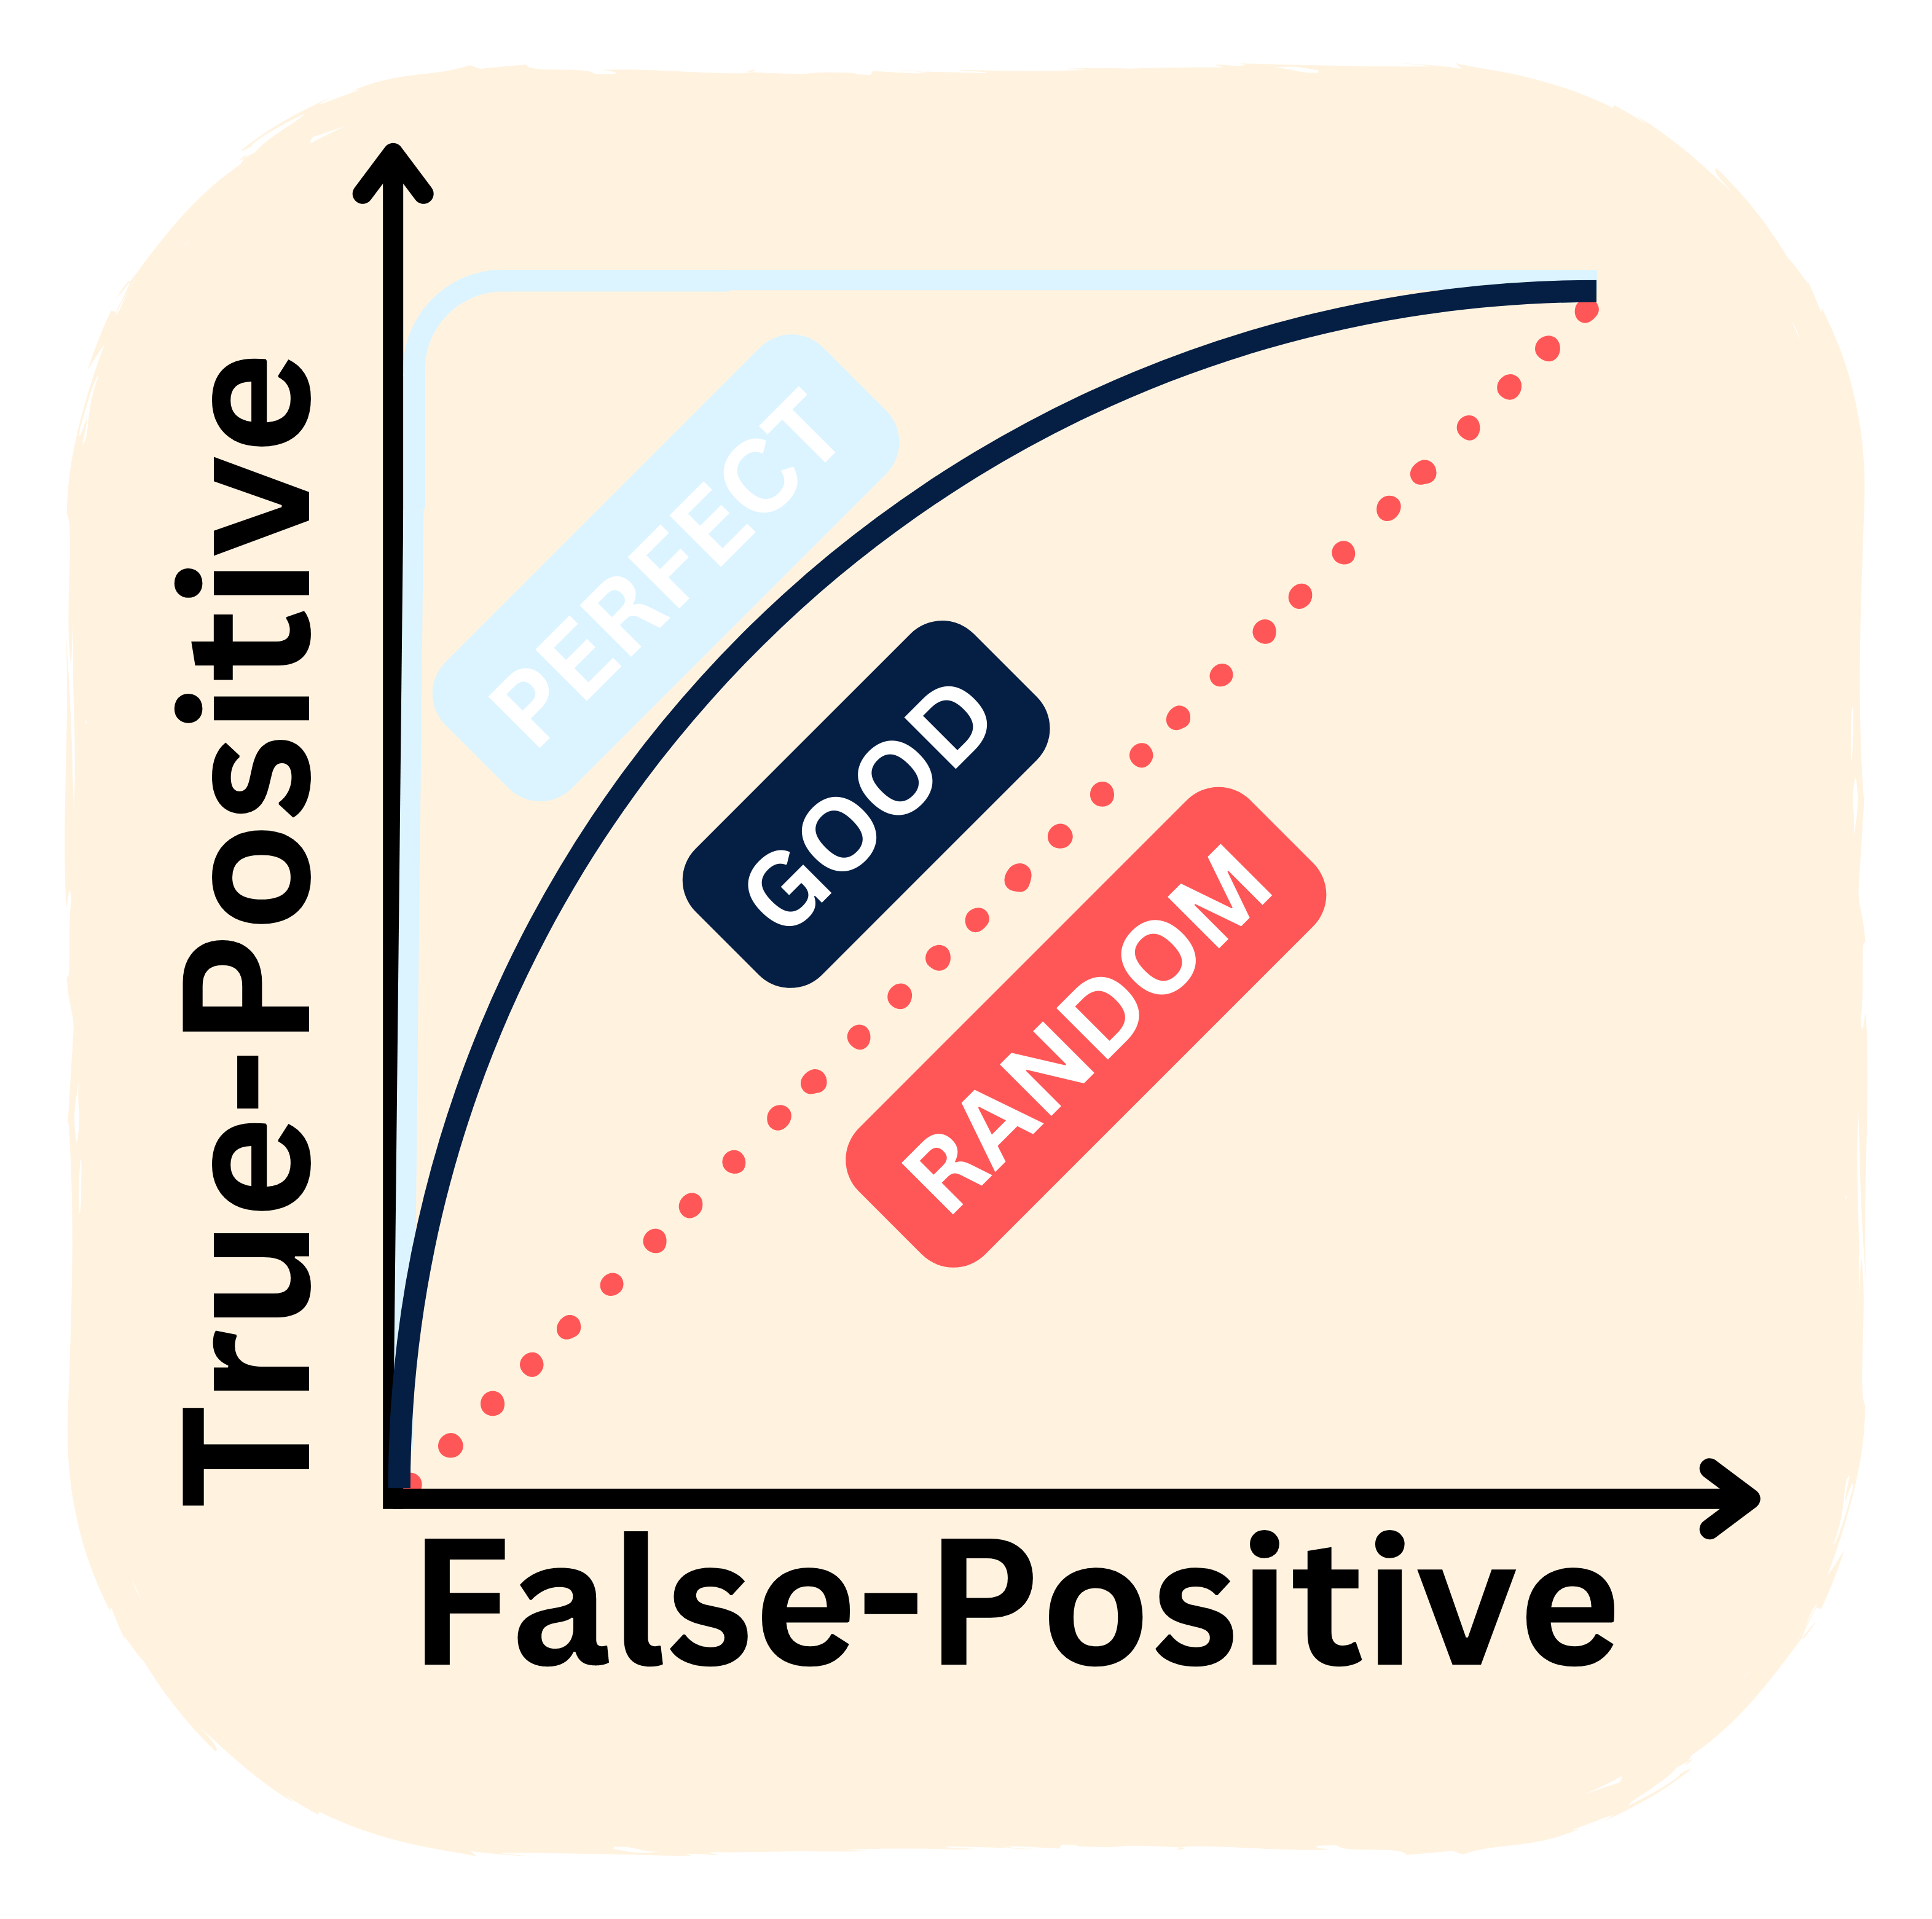
\includegraphics[width=0.45\textwidth]{Figures/Illustrations/True-Positive.png}
    }
    \caption{An illustration of a ROC curve.}
    \label{fig:ROC}
\end{figure}
\subsection{Interpretability}


\subsection{Generalizability}